\documentclass[10pt,twocolumn]{article}
\usepackage[margin=.75in]{geometry}
\usepackage[english]{babel}
\usepackage{amssymb}
\usepackage{amsmath}
\usepackage{multicol}
\usepackage{blindtext}
\usepackage{gensymb}
\usepackage{multirow}
\usepackage{graphicx}
\graphicspath{{./figures/}}
\usepackage{hyperref}
\usepackage{psfrag}
\usepackage{pstool}

\usepackage{pgfplots} 

\pgfplotsset{compat=newest} 
\pgfplotsset{plot coordinates/math parser=false} 
\newlength\figureheight 
\newlength\figurewidth 
%% Page numbering # of ## bottom right of page
\usepackage{lastpage}
\usepackage{fancyhdr}
\pagestyle{fancy}
\fancyhf{}
\renewcommand{\headrulewidth}{0pt}
\rfoot{\thepage\ of \pageref{LastPage}}

\begin{document}

\twocolumn[
\begin{@twocolumnfalse}
\hrule width \hsize height 2pt \vspace{1pt} \hrule width \hsize \kern 1mm
\vspace{1mm}
{\centering
\Large\textbf{{Trials and Tribulations of a\\ Thermal Model for Printed Circuit Board\\ with Internal Heat Generation}}
\vspace{1mm}
\hrule width \hsize \kern 1pt
\vspace{1mm}

\normalsize
{\centering
    \begin{tabular}{ r l }
        Dr. Rico A. R. Picone & Jonathon R. Carstens
    \end{tabular}\par}

\textit{Department of Mechanical Engineering, Saint Martin's University}\\
\today
\par}
\vspace{1mm}

\hrule width \hsize \kern 1pt \hrule width \hsize height 2pt

\begin{abstract}
\noindent
\blindtext
\end{abstract}
\vspace{1mm}
\hrule width \hsize \kern 1pt
\vspace{5mm}
\end{@twocolumnfalse}
]

\section{Early Days}
Currently there exists a problem with the model where the corner elements desperately want to be 0 degrees. \autoref{fig:TempResponse0} shows the temperatures of the center and four corner elements against time. In this simulation, an element that is one diagonal unit toward the center of the plate, in the direction of the center of the plate, is powered. The edges, top, and bottom of the plate should be adiabatic. Power is input into the simulation for half the simulation time. \autoref{fig:TempResponse0} shows the temperature of the closest corner element reaching an elevated temperature quickly and increasing until the point which power is turned off. At this time, the temperature of the corner element dives to meet with the other three corners and begins approaching 0 degrees. The center element can be seen doing the same thing, but with an offset. \autoref{fig:ContourTrans0} shows transient contour plots of the simulation. The same behavior is shown. Setting the input to a negative number, or cooling the node down, exhibits exactly the same behavior. The node will cool while the input is active, but will immediately begin approaching 0 degrees when the input is turned off.

\section{June 28}
More troubleshooting completed on the thermal model. Comments added to the MATLAB code to make it more clear what each section does and make it (hopefully) more readable. I built a new set of figures, \autoref{fig:TempResponse,it20,pi-100} and \autoref{fig:ContourTrans,it20,pi-100} which show what happens when the model is started with an initial temperature and allowed to run to the point which the asymptotic behavior of the temperature response is evident. So I now know for certain that the model is approaching 0 degrees and not the initial temperature (which was 0 degrees before and had me skeptical). I still plan on using a $3\times3$ element plate to run through the creation of \textbf{A} and \textbf{B} to see if they are being created in MATLAB the way I think they should be. I don't know if rebuilding the matrix generation in another program (Mathematica or Python) will be a good idea. If there is an error in my MATLAB code, I probably wouldn't see if using another syntax to recreate the code. I'd likely run into a whole new set of syntax problems there, and it might be easy enough to just do it on paper for a model with 9 nodes. I will start wading into that and see what comes out of it.

\section{June 29}
The problem with the corners was fixed last night. Writing the $3\times3$ \textbf{A} and \textbf{B} matrices made me realize that it was an error with the coefficient values on the MATLAB code. I had left out lines in the code that would change the coefficients of the corners to their intended values, so they stayed the same as the edge elements, which caused them to be broken. Now heat does not dump out of the corners and the model seems to be behaving as it should. The next step is to verify that it follows the laws of heat transfer. This is going to be checked by using a known analytic case with a solution as well as checking that energy is conserved when heat is put into the system. \autoref{fig:TmpRspn25x25,15Wleftedge,-15Wrightedge} shows the temperature response of the plate when equal power is applied and removed from the left and right edges of the plate. The center of the plate holds a steady temperature, while a nice temperature gradient forms through the plate. This indicates to me that heat transfer is working well and the inputs and outputs are at least working evenly, if not correctly. The analytic solution should tell if heat transfer is working \textbf{correctly}. One quick check was done to see what happens when the same 15 watt input and sink is started at $t_{init}$ and stopped half way through the simulation. The temperature response for this simulation is shown in \autoref{fig:TmpRspn25x25,15Wleftedge,-15Wrightedge,halftime}. The plot shows that the plate builds a temperature gradient across it's width, and returns to the initial temperature when the power inputs are stopped. My intuition says that this is an early indication of energy conservation.

\section{October 4}
Revised mathematical equations so that heat transfer from the top and bottom of the elements are controlled by convection instead of a constant power input. This puts those sources into the A matrix. $Q_{OT}$ and $Q_{OB}$ are now $Q_{s} = h_{t}AT_{c}$ and $Q_{s} = h_{b}AT_{c}$, respectively.

\section{October 22}
Created GitHub repository and uploaded files, including an old April version of the thermal model. Initial test of that file showed that it didn't run. Not sure what the problem was, but it should be easy to get that code working if there is a need for an earlier version.

\section{October 25}
Thermal model was broken for a short time while I changed too much in an initial attempt to convert power output to convection. I was able to get the model back into a working state, but I still need to check that everything is functioning as it should again. This problem occurred during the October 4th update, and motivated the GitHub addition to help with revision and change control.

\section{Introduction}
The objective of this paper is to develop and simulate a two dimensional mathematical thermal model for a laminate printed circuit board (PCB) with internal heat generation. The PCB is constructed of layers of FR4 and etched copper laminated together. As shown in \autoref{fig:pcb}, there are multiple, alternating layers of FR4 and etched copper within the PCB. The PCB will generate heat through internally printed copper circuit layers when power is applied to the circuit. The PCB will be simulated as powered in still room temperature air, where the only heat loss is due to convection from the surface of the PCB. The top, bottom, and side surfaces of the PCB are subject to heat loss, however the PCB is very thin compared to its length and width, so it may be simulated as adiabatic along its edge.

\section{Discrete Model}
The PCB is modeled as a discrete finite elements model with $n \times m$ square nodes. Each node represents a thermal capacitance of the PCB layers and is connected to each other node directly adjacent to it by a thermal resistance. Each node is capable of independent internal heat generation and features independent heat loss through the top and bottom. The edge and corner nodes also feature heat loss through the side of the PCB.

\begin{figure}
	\center
	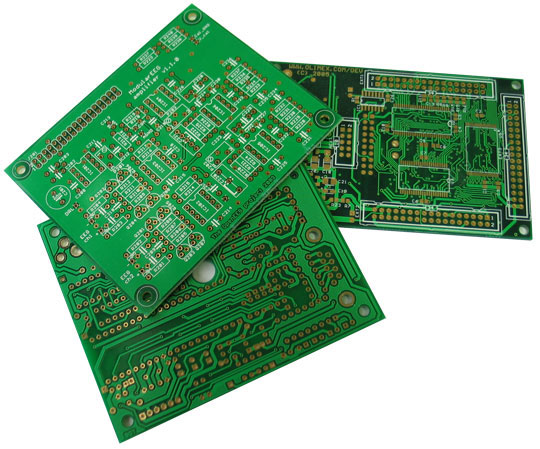
\includegraphics[width=0.6\linewidth]{pcb}
	\caption{Stand-in for a PCB layer diagram.}
	\label{fig:pcb}
\end{figure}

\begin{figure}
	\center
	\includegraphics[width=0.8\linewidth]{TempResponse0.eps}
	\caption{Temperature response for five elements in model with 0 degree initial temperature and 7 watt input to a single element in the lower left corner. All controllable sources of heat loss are set to 0. \textbf{The model is broken at this time.}}
	\label{fig:TempResponse0}
\end{figure}

\begin{figure}
	\center
	\includegraphics[width=0.8\linewidth]{TempResponse22.eps}
	\caption{Temperature response for five elements in model with 22 degree initial temperature and 7 watt input to a single element in the lower left corner. All controllable sources of heat loss are set to 0. \textbf{The model is broken at this time.}}
	\label{fig:TempRespsonse22}
\end{figure}

\begin{figure}
	\center
	\includegraphics[width=0.8\linewidth]{TempResponse,it20,pi-100.eps}
	\caption{Temperature response for five elements in model with 20 degree initial temperature and -100 watt input to a single element in the center of plate. All controllable sources of heat loss are set to 0. Temperature of plate starts at a uniform 20 degrees, begins to drop due to 100 watt power loss at the center. Power input is turned off at $t=1/10\ t_{max}$ through the simulation which causes the model to react by approaching 0 degrees. Note: All four corners track along the same time/temp profile causing them to appear as one curve on this plot. \textbf{The model is broken at this time.}}
	\label{fig:TempResponse,it20,pi-100}
\end{figure}

\begin{figure}
	\center
	\includegraphics[width=0.8\linewidth]{TmpRspn25x25,15Wleftedge,-15Wrightedge.eps}
	\caption{Temperature response for five elements in model with 20 degree initial temperature. 15 watts total is applied to the left edge of the plate. 15 watts total are drawn from the right edge of the plate. All other surfaces of the plate are adiabatic. The simulation is ran for 1800 seconds to achieve steady state.}
	\label{fig:TmpRspn25x25,15Wleftedge,-15Wrightedge}
\end{figure}

\begin{figure}
	\center
	\includegraphics[width=0.8\linewidth]{TmpRspn25x25,15Wleftedge,-15Wrightedge,halftime.eps}
	\caption{Temperature response for five elements in model with 20 degree initial temperature. 15 watts total is applied to the left edge of the plate. 15 watts total are drawn from the right edge of the plate. All other surfaces of the plate are adiabatic. Power input and loss is stopped one third of the way through the simulation time. The simulation is ran for 1800 seconds to achieve steady state.}
	\label{fig:TmpRspn25x25,15Wleftedge,-15Wrightedge,halftime}
\end{figure}


\begin{figure}
	\center
	\includegraphics[width=0.8\linewidth]{ContourTrans0.eps}
	\caption{Contour plots of model during four time steps. Same simulation parameters as \autoref{fig:TempResponse0} \textbf{The model is broken at this time.}}
	\label{fig:ContourTrans0}
\end{figure}


\begin{figure}
	\center
	\includegraphics[width=0.8\linewidth]{ContourTrans,it20,pi-100.eps}
	\caption{Contour plots of model during four time steps. Same simulation parameters as \autoref{fig:TempResponse,it20,pi-100} \textbf{The model is broken at this time.}}
	\label{fig:ContourTrans,it20,pi-100}
\end{figure}


\begin{figure}
	\center
	\includegraphics[width=0.8\linewidth]{CtrTnst25x25,15Wleftedge,-15Wrightedge.eps}
	\caption{Contour plots of model during four time steps. Same simulation parameters as \autoref{fig:TmpRspn25x25,15Wleftedge,-15Wrightedge}}
	\label{fig:CtrTnst25x25,15Wleftedge,-15Wrightedge}
\end{figure}


\begin{figure}
	\center
	\includegraphics[width=0.8\linewidth]{CtrTnst25x25,15Wleftedge,-15Wrightedge,halftime.eps}
	\caption{Contour plots of model during four time steps. Same simulation parameters as \autoref{fig:TmpRspn25x25,15Wleftedge,-15Wrightedge,halftime}}
	\label{fig:CtrTnst25x25,15Wleftedge,-15Wrightedge,halftime}
\end{figure}

\twocolumn
\section{Equations}
\subsection{Internal Element}
\begin{equation}
\begin{split}
\dot{T}_{c_{i,j}} 	& = \frac{1}{c_{i,j}}
					\Biggl[\Biggr.
					 	Q_{I_{i,j}} + h_{t}AT_{c_{i,j}} + h_{b}AT_{c_{i,j}} \\					
					&	- \frac{1}{R_{i+1,j,1}}\left(T_{c_{i,j}}- T_{c_{i,j-1}}\right) \\
					& 	- \frac{1}{R_{i,j+1,2}}\left(T_{c_{i,j}}- T_{c_{i-1,j}}\right) \\
					& 	- \frac{1}{R_{i+1,j+1,1}}\left(T_{c_{i,j}}- T_{c_{i,j+1}}\right) \\
					& 	- \frac{1}{R_{i+1,j+1,2}}\left(T_{c_{i,j}}- T_{c_{i+1,j}} + \right)
					\Biggl.\Biggl]
\end{split}
\end{equation}

\subsection{Top Edge Element}
\begin{equation}
\begin{split}
\dot{T}_{c_{1,j}}	& = \frac{1}{c_{1,j}}
					\Biggl[\Biggr.
					 	   Q_{OS_{1,j+1}} \\
					&	 + Q_{I_{1,j}}+ h_{t}AT_{c_{1,j}} + h_{b}AT_{c_{1,j}} \\
					&	- \frac{1}{R_{2,j,1}}\left(T_{c_{1,j}}- T_{c_{1,j-1}}\right) \\
					& 	- \frac{1}{R_{2,j+2,2}}\left(T_{c_{1,j}}- T_{c_{2,j}}\right) \\
					& 	- \frac{1}{R_{2,j+1,1}}\left(T_{c_{1,j}}- T_{c_{1,j+1}}\right)
					\Biggl.\Biggr]
\end{split}
\end{equation}

\subsection{Left Edge Element}
\begin{equation}
\begin{split}
\dot{T}_{c_{i,1}}	& = \frac{1}{c_{i,1}}
					\Biggl[\Biggr.
					 	  Q_{OS_{i+1,1}} \\
					&	+ Q_{I_{i,1}}+ h_{t}AT_{c_{i,1}} + h_{b}AT_{c_{i,1}} \\
					&	- \frac{1}{R_{i,2,2}}\left(T_{c_{i,1}}- T_{c_{i-1,1}}\right) \\
					& 	- \frac{1}{R_{i+1,2,1}}\left(T_{c_{i,1}}- T_{c_{i,2}}\right) \\
					& 	- \frac{1}{R_{i+1,2,2}}\left(T_{c_{i,1}}- T_{c_{i+1,1}}\right)
					\Biggl.\Biggr]
\end{split}
\end{equation}

\subsection{Right Edge Element}
\begin{equation}
\begin{split}
\dot{T}_{c_{i,m}}	& = \frac{1}{c_{i,m}}
					\Biggl[\Biggr.
					 	  Q_{OS_{i+1,m+1}} \\
					&	+ Q_{I_{i,m}}+ h_{t}AT_{c_{i,m}} + h_{b}AT_{c_{i,m}} \\					
					&	- \frac{1}{R_{i,m+1,2}}\left(T_{c_{i,m}}- T_{c_{i-1,m}}\right) \\
					& 	- \frac{1}{R_{i+1,m,1}}\left(T_{c_{i,m}}- T_{c_{i,m-1}}\right) \\
					& 	- \frac{1}{R_{i+1,m+1,2}}\left(T_{c_{i,m}}- T_{c_{i+1,m}}\right)
					\Biggl.\Biggr]
\end{split}
\end{equation}

\subsection{Bottom Edge Element}
\begin{equation}
\begin{split}
\dot{T}_{c_{n,j}}	& = \frac{1}{c_{n,j}}
					\Biggl[\Biggr.
					 	   Q_{OS_{n+2,j+1}} \\
					&	 + Q_{I_{n,j}}+ h_{t}AT_{c_{n,j}} + h_{b}AT_{c_{n,j}} \\
					&	- \frac{1}{R_{n+1,j,1}}\left(T_{c_{n,j}}- T_{c_{n,j-1}}\right) \\
					& 	- \frac{1}{R_{n,j+1,2}}\left(T_{c_{n,j}}- T_{c_{n-1,j}}\right) \\
					& 	- \frac{1}{R_{n+1,j+1,1}}\left(T_{c_{n,j}}- T_{c_{n,j+1}}\right)
					\Biggl.\Biggr]
\end{split}
\end{equation}

\subsection{Top Left Corner Element}
\begin{equation}
\begin{split}
\dot{T}_{c_{1,1}}	& = \frac{1}{c_{1,1}}
					\Biggl[\Biggr.
					 	  Q_{OS_{2,1}} + Q_{OS_{1,2}} \\
					& 	+ Q_{I_{1,1}}+ h_{t}AT_{c_{1,1}} + h_{b}AT_{c_{1,1}} \\
					&	- \frac{1}{R_{2,2,2}}\left(T_{c_{1,1}}- T_{c_{2,1}}\right) \\
					& 	- \frac{1}{R_{2,2,1}}\left(T_{c_{1,1}}- T_{c_{1,2}}\right)
					\Biggl.\Biggr]
\end{split}
\end{equation}

\subsection{Top Right Corner Element}
\begin{equation}
\begin{split}
\dot{T}_{c_{1,m}}	& = \frac{1}{c_{1,m}}
					\Biggl[\Biggr.
					 	  Q_{OS_{2,m+2}} + Q_{OS_{1,m+1}} \\
					& 	+ Q_{I_{1,m}}+ Qh_{t}AT_{c_{1,m}} + h_{b}AT_{c_{1,m}} \\
					&	- \frac{1}{R_{2,m,1}}\left(T_{c_{1,m}}- T_{c_{1,m-1}}\right) \\
					& 	- \frac{1}{R_{2,m+1,2}}\left(T_{c_{1,m}}- T_{c_{2,m}}\right)
					\Biggl.\Biggr]
\end{split}
\end{equation}

\subsection{Bottom Left Corner Element}
\begin{equation}
\begin{split}
\dot{T}_{c_{n,1}}	& = \frac{1}{c_{n,1}}
					\Biggl[\Biggr.
					 	  Q_{OS_{n+1,1}} + Q_{OS_{n+2,2}} \\
					& 	+ Q_{I_{n,1}}+ h_{t}AT_{c_{n,1}} + h_{b}AT_{c_{n,1}} \\
					&	- \frac{1}{R_{n,2,2}}\left(T_{c_{n,1}}- T_{c_{n-1,1}}\right) \\
					& 	- \frac{1}{R_{n+1,2,1}}\left(T_{c_{n,1}}- T_{c_{n,2}}\right) 
					\Biggl.\Biggr]
\end{split}
\end{equation}

\subsection{Bottom Right Corner Element}
\begin{equation}
\begin{split}
\dot{T}_{c_{n,m}}	& = \frac{1}{c_{n,m}}
					\Biggl[\Biggr.
						  Q_{I_{n,m}}+ h_{t}AT_{c_{n,m}} + h_{b}AT_{c_{n,m}} \\
					&	+ Q_{OS_{n+1,m+2}} + Q_{OS_{n+2,m+1}} \\
					&	- \frac{1}{R_{n,m+1,2}}\left(T_{c_{n,m}}- T_{c_{n-1,m}}\right) \\
					& 	- \frac{1}{R_{n+1,m,1}}\left(T_{c_{n,m}}- T_{c_{n,m-1}}\right)
					\Biggl.\Biggr]
\end{split}  
\end{equation}

\begin{table}[htbp]
\center
	\begin{tabular}{ l r l}
		\multicolumn{3}{l}{Kawasaki KX250F Engine Parameters} \\ \hline
		Number of Cylinders & $1$ &\\
		Number of Cycles & $4$ &\\
		Bore & $77.0$ & $mm$\\
		Stroke & $53.6$ & $mm$\\ 
		Displacement & $249$ & $cc$\\ 
		Connecting Rod Length & $92.5$ &$mm$\\
		Compression Ratio & 13.8:1 & \\
	\end{tabular}
	\caption{Sample for table formatting.}
	\label{tab:engine}
\end{table}



\end{document}